\chapter{\label{chap:state}Bestehende offlinefähige Systeme / Konzepte}
%
% Software
%
\section{Kollaborative Software}
  \highlight{rauslassen?}
  Kann ich benutzen um kollaborativ zu arbeiten --> \b{was passiert wenn ich offline bin?}
  \sub{Google Docs}
  (benutzt OT)
  \sub{Google Wave}
  (benutzt OT)
  \sub{Dropbox / 'Clouds'}
  \sub{Kollaborative Editoren}
  Wiki: \url{https://en.wikipedia.org/wiki/Collaborative_real-time_editor}\\\\
  \url{https://atom.io/packages/covalent}\\
  \url{https://atom.io/packages/firepad}\\
  Markdown: \url{https://hackmd.io/}\\
  LaTeX: \url{https://www.sharelatex.com/}\\
  Online editor: \url{http://etherpad.org/} (OT)\\
  Mockingbird (tool for creating wireframes): \url{https://gomockingbird.com/home} (OT)\\
  marvelapp? \url{https://marvelapp.com/collaboration/}

  --> Zahl steigend, (nachdem Google die Drive Realtime API veröffentlicht hat, die auf \gls{OT} basiert und es \it{third-party Apps} ermöglicht, dieselbe Zusammenarbeit wie Google Docs zu verwenden)\\\\
  \b{plus} wachsende Anzahl von offen zur Verfügung gestellter Bibliotheken und Frameworks die es ermöglichen, offlinefähige Anwendungen zu programmieren. Siehe Kapitel \ref{sec:frameworks}
%
% Frameworks / Bibliotheken
%
\section{\label{sec:frameworks}Offline-First Frameworks/Bibliotheken}
  Ich möchte aber auch eigenständig Software entwickeln die man vielleicht nicht nur zum Arbeiten nehmen kann, sondern auch um Quatsch zu machen wie Katzengifs zu teilen.
  \sub{redux? react-native? webpack?}
  \Gls{PWA}
  %
  % realm
  %
  \sub{Realm}
  %
  % Datomic
  %
  \sub{Datomic? (Closure)}
  \cite{realm}
  %
  % redux-offline
  %
  \sub{Redux Offline}
  ``Persistenter Redux store für \it{reasonaboutable}\texttrademark ~Offline-First Anwendungen``. \\
  Ist ein eigenständiger Statuscontainer und kann mit jeder Webanwendung angewandt werden, die sich \it{deklarativ auf Basis einer einzigen Datenquelle rendern lässt}, wie beispielsweise React\footnote{JavaScript Bibliothek: \url{https://reactjs.org/}}, Vue\footnote{JavaScript Framework: \url{https://vuejs.org/}}, oder Angular\footnote{JavaScript Framework: \url{https://www.angular.io}}~\cite{redux-offline-compabilaty}.\\
  ist eine experimentelle Bibliothek die die Offline-First Architektur implementiert?\\
  \sc{Redux Offline} verspricht nicht, die Webanwendung offlinefähig zu machen. Um \it{assets}(Bilder, Skripte etc) zwischenzuspeichern, muss zusätzlich noch ein ServiceWorker implementiert sein.\\
  Benutzt redux-persist und redux-optimist.\\
  Bei jeder Änderung wird der Redux store auf dem Datenträger gespeichert, und bei jedem Start automatisch neugeladen. (Standardmäßig IndexedDB, localForage, AsyncStorage)\\
  Eine mit \sc{Redux Offline} erstellte Anwendung funktioniert ohne weitere Anpassung offline im Lesemodus. Also wenn die benutzende Person vom (Redux-)Status lesen möchte.
  Um auch im Schreibmodus offline zu funktionieren, werden alle Netzwerkgebundenen Aktionen in einem Store-internem \gls{Queue} gespeichert. Dann erstellt \sc{Redux Offline} einen Unterbaum \tt{offline}, wo unter anderem der internen Status und ein Array namens \tt{outbox} verwaltet wird. Um diese Aktivitäten bei Internetverbindung ausführen zu können, müssen alle notwendigen Daten Plus Metadaten gespeichert werden. Die Metadaten sind für die Information zuständig, was davor oder danach passieren soll. Es gibt drei Metadaten die \sc{Redux Offline} interpretieren kann:\\
  \tt{meta.offline.effect} - Die Daten die gesendet werden sollen?\\
  \tt{meta.offline.commit} - Aktion die ausgeführt wird sobald Daten erfolgreich gesendet wurden\\
  \tt{meta.offline.rollback} - Aktion die bei permanent fehlgeschlagener Internetverbindung
  ~\cite{redux-offline-gh}
  \begin{figure}[H]
    \centering
    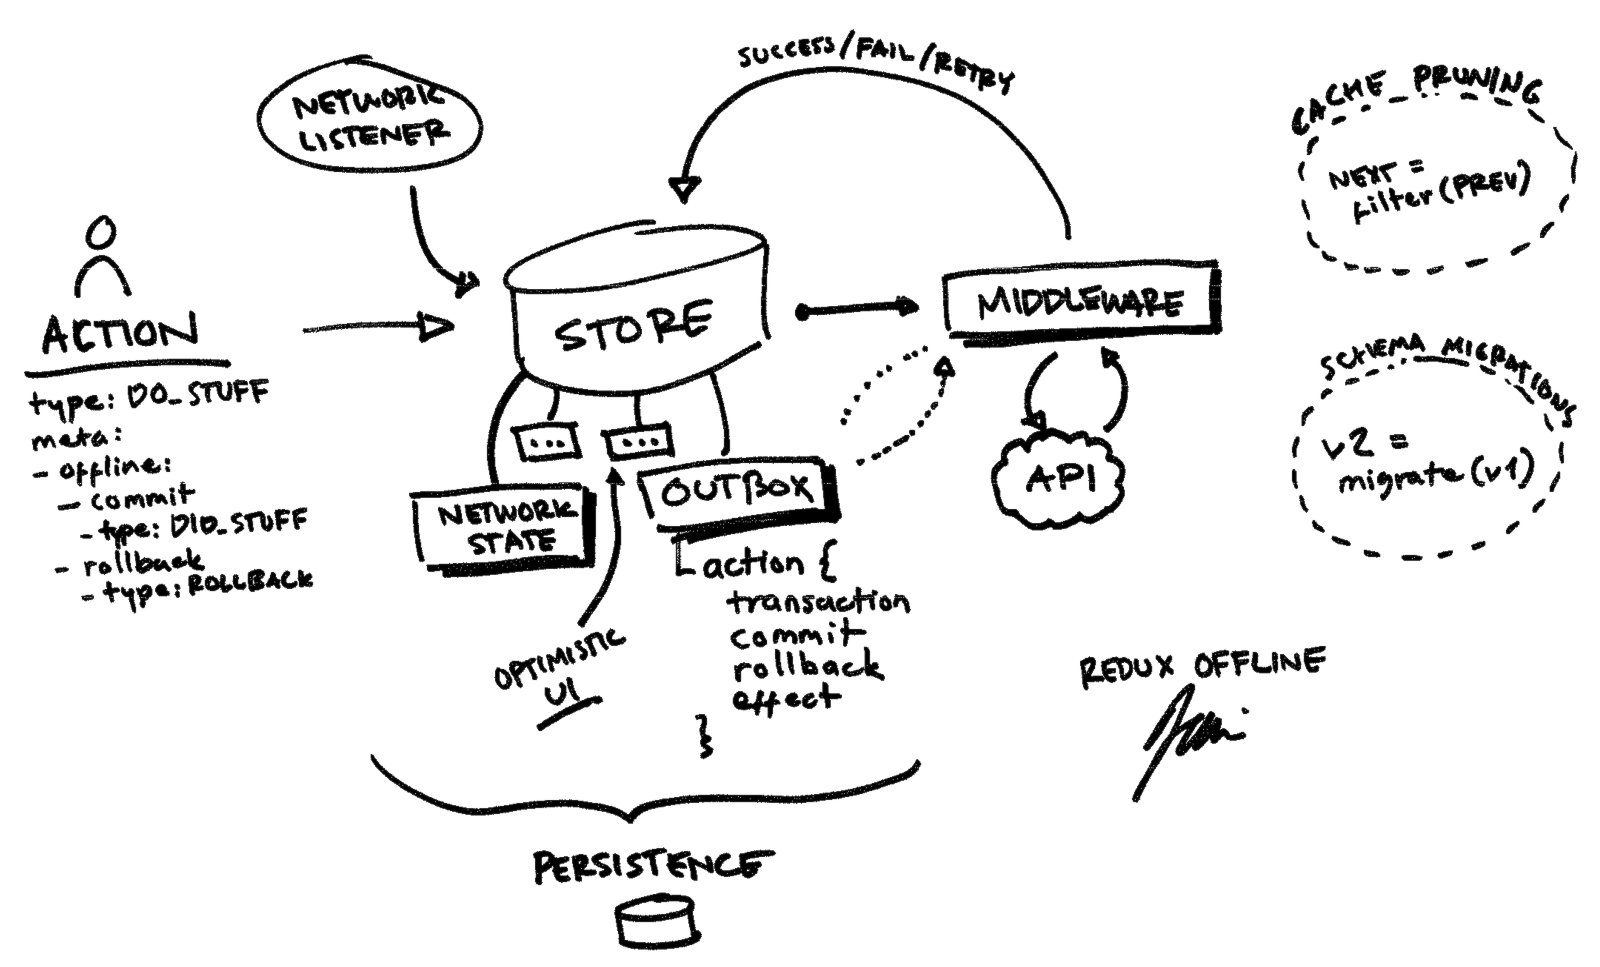
\includegraphics[width=\textwidth]{redux-offline}
    \grayRule
    \caption[Redux Offline]{Redux Offline Architektur\\\\~Quelle:~\cite{redux-offline}}
     \label{fig:redux-offline}
\end{figure}
Die grundlegende Idee hinter Redux Offline ist, dass der \sc{Redux store} die Datenbank ersetzt/ist. Jede Aktion die benötigt wird um offline zu arbeiten, wird im \sc{store} persisiert und durch die \tt{meta.offline} -Daten weiß die Anwendung was online zu tun ist. Wie die Grafik \ref{fig:redux-offline} (links) zeigt, wird jede (offline-unterstützende) Aktion mit dem \tt{offline.meta} Feld dekoriert. Darin wird beschrieben, wie der \it{Netzwerkeffekt} ausgeführt werden soll (\tt{effect}) und welche Aktion ausgelöst werden soll, wenn sie erfolgreich (\tt{commit}) ist oder fehlschlägt (\tt{rollback}). Diese Offline-Aktionen werden im \sc{store}-internen \gls{Queue} gespeichert und werden, einmal online, an den Server gesendet. \gls{UI} \gls{optimistic UI}\\

{\LARGE Konflikte?}
  %
  % redux persist
  %
  \subsub{redux-persist}
  localStorage. github~\cite{redux-persist-gh} medium~\cite{redux-persist}
  \subsub{redux-optimist}
  %
  % react-native-offline
  %
  \sub{react-native-offline}
  github \cite{rn-offline-gh} medium\cite{rn-offline-medium}
  %
  % webpack offline-plugin
  %
  \sub{offline-plugin für webpack}
  github\cite{webpack-gh}
  dev\cite{webpack-dev}
  %
  % hoodie
  %
  \sub{hoodie}
  \cite{hoodie}